\chapter{Introduction}
\section{Multipath in Aeronautical Telemetry}
Multipath interference is one of the dominant causes for link loss in aeronautical telemetry.
Strong multipath interference occurs when the transmitted signal is received via multiple paths when a test article is in a low elevation angle scenario, as shown in Figure \ref{fig:multipath}.
Multipath propagation is modeled as linear, time-invariant system with a finite length impulse response.
Equalizers have been studied to combat this form of multipath interference in aeronautical telemetry \cite{rice-afran-saquib:2014,rice-afran-saquib-cole-rhodes-moazzami:2014}.
There are two general classes of equalizers, blind and data-aided.
Blind equalizers are adaptive filters whose coefficient update algorithm is based on the known statistical properties of the transmitted signal, but have no knowledge of the specific data or multipath channel is assumed.
Data-aided equalizers are also filters whose impulse responses are calculated from the propagation conditions.
One method of obtaining an estimate of this knowledge is to periodically insert a known bit sequence called a ``pilot'' into the data stream.
The receiver compares the received signal corresponding to the pilot with a locally stored copy to estimate parameters such as the multipath channel, frequency offset, phase offset, and noise variance.
\begin{figure}
	\centering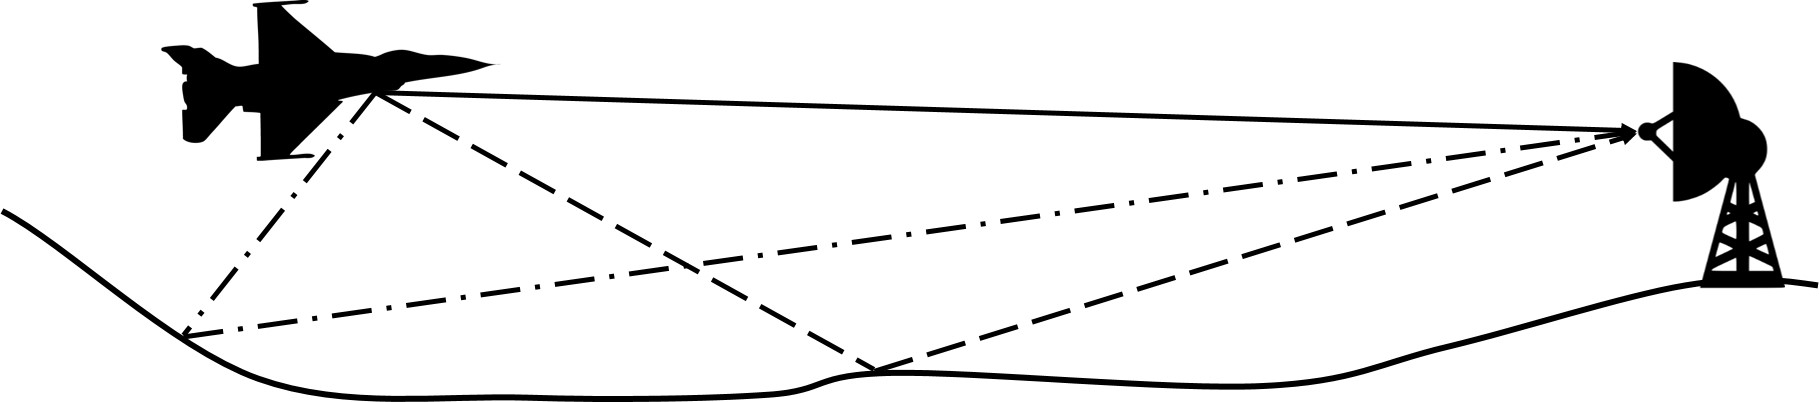
\includegraphics[width=12.11in/100*50]{figures/intro/Picture1.jpg}
	\caption{Multipath interference can occur when a signal is received from multiple paths.}
	\label{fig:multipath}
\end{figure}
\section{Problem Statement}
The real-time signal processing for a digital communications system with data-aided equalizers is computationally heavy.
Digital communication algorithms implemented in a high performance Central Processing Unit (CPU) cannot meet the real-time requirement.
Graphic Processing Units (GPUs) can be used to perform real-time processing because of their massively parallel architecture.

This thesis studies how signal processing can be reformulated to run quickly and efficiently in GPUs.
Optimized libraries harness GPU resources to make signal processing implementation relatively easy and extremely fast.
%Processing signals in batches to introduce more parallelism.
If algorithms can be reformulated for batch processing and use matrix/vector multiplication or Fast Fourier Transform libraries, GPUs can provide vast speed ups.

\section{Organization}
Chapter \ref{chap:PAQ_project} describes the Preamble Assisted Equalization (PAQ) system and introduces the digital signal processing algorithms.
Chapter \ref{chap:gpu} provides an overview of signal processing in GPUs.
Chapter \ref{chap:equalizers_in_gpus} describes how the five equalizers are implemented in GPUs.
The thesis concludes with the summary and conclusions in Chapter \ref{chap:final_summary}.